\documentclass[tikz,border=14pt]{standalone}
\usepackage[T1]{fontenc}
\definecolor{espresso}{HTML}{A65032}
\definecolor{milk}{HTML}{267C70}
\definecolor{cold}{HTML}{346CB0}
\definecolor{sugar}{HTML}{AC7620}
\definecolor{decaf}{HTML}{8254A0}
\begin{document}
% Five circles have at most n(n-1)+2 = 22 plane regions,
% including the exterior. Thus a 31-region Venn diagram is impossible.
% These circles are in general position and attain 21 interior regions.
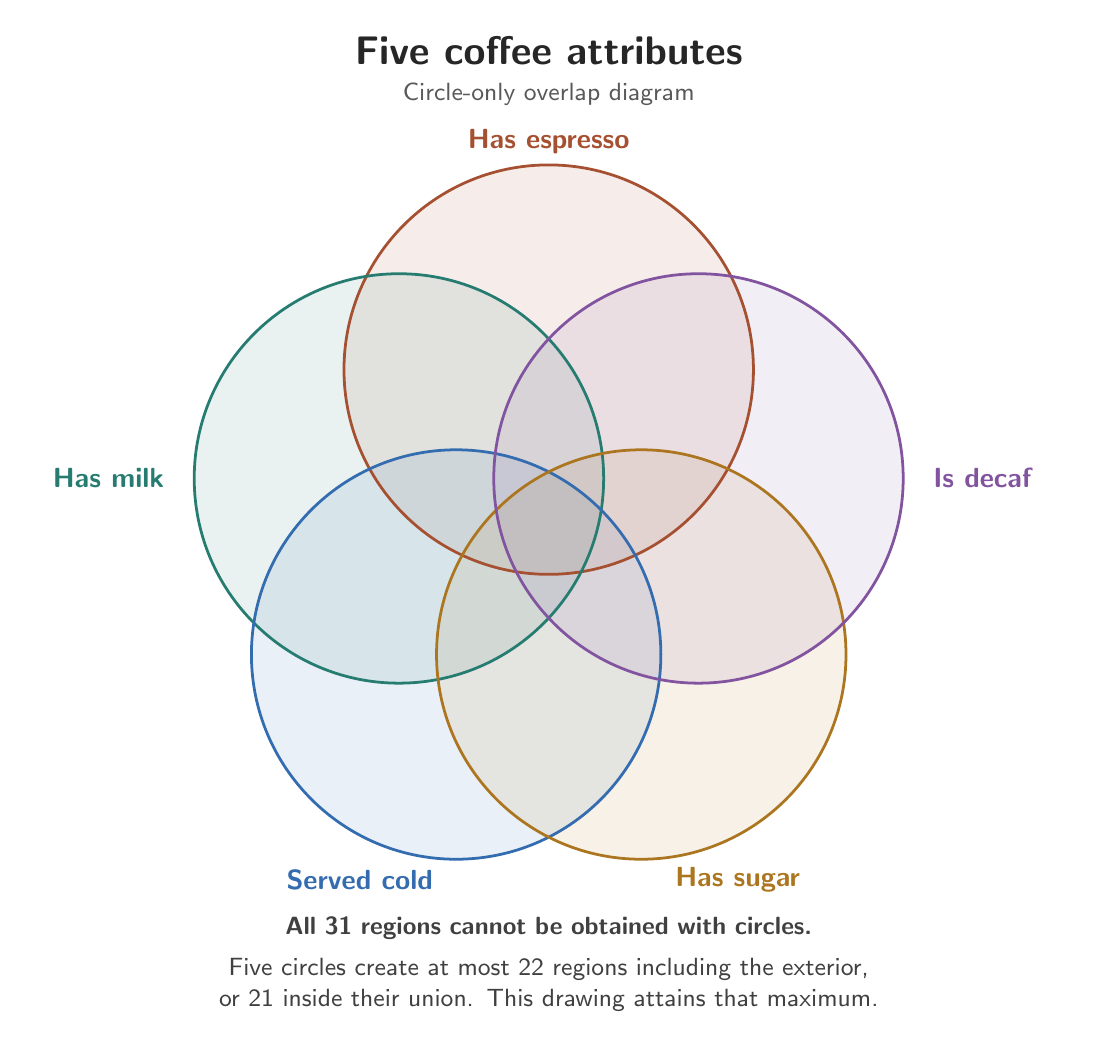
\begin{tikzpicture}[font=\sffamily, line width=1pt]
  \node[font=\sffamily\bfseries\Large, text=black!85] at (0,6.05)
    {Five coffee attributes};
  \node[font=\sffamily\small, text=black!65] at (0,5.50)
    {Circle-only overlap diagram};

  \coordinate (A) at (90:2);
  \coordinate (B) at (162:2);
  \coordinate (C) at (234:2);
  \coordinate (D) at (306:2);
  \coordinate (E) at (18:2);
  % Fill first, then redraw every boundary so none is obscured.
  \foreach \p/\c in {A/espresso,B/milk,C/cold,D/sugar,E/decaf}
    \fill[\c,fill opacity=.10] (\p) circle[radius=2.6];
  \foreach \p/\c in {A/espresso,B/milk,C/cold,D/sugar,E/decaf}
    \draw[\c] (\p) circle[radius=2.6];

  \node[text=espresso,font=\sffamily\bfseries] at (0,4.90) {Has espresso};
  \node[text=milk,font=\sffamily\bfseries,anchor=east] at (-4.75,.62) {Has milk};
  \node[text=cold,font=\sffamily\bfseries] at (-2.40,-4.48) {Served cold};
  \node[text=sugar,font=\sffamily\bfseries] at (2.40,-4.48) {Has sugar};
  \node[text=decaf,font=\sffamily\bfseries,anchor=west] at (4.75,.62) {Is decaf};

  \node[align=center,text=black!75,font=\sffamily\small,text width=13cm] at (0,-5.55)
    {\textbf{All 31 regions cannot be obtained with circles.}\\[4pt]
     Five circles create at most 22 regions including the exterior,\\
     or 21 inside their union. This drawing attains that maximum.};
\end{tikzpicture}
\end{document}
